%%%%%%%%%%%%%%%%%%%%%%%%%%%%%%%%%%%%%%%%%%%%%%%%%%%%%%%%%%%%%%%%%%%%%%%%%%%%%%%%
% binary_search_tree.tex
% An example demonstrating how to create a binary search tree in LaTeX with TikZ
% Technically, this is an AVL tree with the balances written in at every node
% https://github.com/mhyee/latex-examples/
%%%%%%%%%%%%%%%%%%%%%%%%%%%%%%%%%%%%%%%%%%%%%%%%%%%%%%%%%%%%%%%%%%%%%%%%%%%%%%%%


% LaTeX Preamble
% Load packages and set options as needed
%%%%%%%%%%%%%%%%%%%%%%%%%%%%%%%%%%%%%%%%%%%%%%%%%%%%%%%%%%%%%%%%%%%%%%%%%%%%%%%%

% Set the document class to "article"
% Pass it "12pt" and "letterpaper" options
\documentclass[12pt,letterpaper]{article}

% We don't need the special font encodings, but still
% good practice to include these. See:
%
% http://tex.stackexchange.com/questions/664/why-should-i-use-usepackaget1fontenc
% http://dsanta.users.ch/resources/type1.html
\usepackage[T1]{fontenc}
\usepackage{ae,aecompl}

% TikZ is what lets us draw graphics
\usepackage{tikz}
% We want to be able to draw split circles
\usetikzlibrary{shapes.multipart}

% Disable page numbering
\pagestyle{empty}


% Define our own macros, for convenience
%%%%%%%%%%%%%%%%%%%%%%%%%%%%%%%%%%%%%%%%%%%%%%%%%%%%%%%%%%%%%%%%%%%%%%%%%%%%%%%%

% \ensuremath{ARG} is used to enable mathematics mode in a macro
% ARG will always be rendered in math mode,
% regardless of which mode the macro is called in
%
% http://www.giss.nasa.gov/tools/latex/ensuremath.html

% \snode{ID}{NUMBER} becomes \node{ID}[item]{\ensuremath{NUMBER}}
\newcommand{\snode}[2]{\node(#1)[item]{\ensuremath{#2}}}

% \avlkey{KEY}{BALANCE} becomes "KEY \nodepart{lower} \ensuremath{BALANCE}}
% Note that \avlkey needs to be placed within a node, eg \node{\avlkey{1}{0}}
\newcommand{\avlkey}[2]{#1 \nodepart{lower} \ensuremath{#2}}

% \avlempty becomes "edge from parent[draw=none]"
\newcommand{\avlempty}{edge from parent[draw=none]}

% Begin the actual typesetting, by starting the "document" environment
%%%%%%%%%%%%%%%%%%%%%%%%%%%%%%%%%%%%%%%%%%%%%%%%%%%%%%%%%%%%%%%%%%%%%%%%%%%%%%%%
\begin{document}

% 93 has just been inserted
% Balances are updated - 91 needs to be balanced
% So the tree looks something like this:
%
%         55
%     38      78
%  12   46   68 91
% 5   43 47 62   92
%                 93
%
% Each node also keeps a "balance"
% balance = height(right) - height(left)

  \begin{center}
    % Set up the options for the diagram
    % - set the distance between levels of the tree
    % - every node is drawn as a (vertically) split circle
    % - "bad" nodes have a 50% opaque red filling
    % - "new" nodes have a 50% opaque green filling
    % - in every level, the distance between siblings is (60 mm)/(level number)
    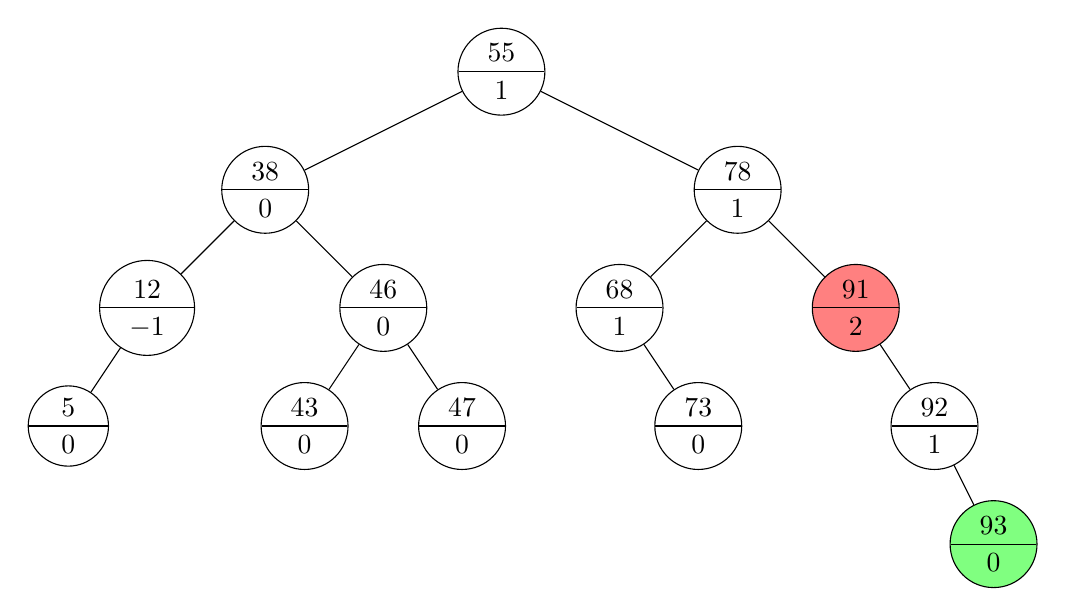
\begin{tikzpicture}[
      level distance=15mm,
      every node/.style={circle,draw,circle split},
      bad/.style={fill=red!50},
      new/.style={fill=green!50},
      level/.style={sibling distance=60mm/#1}
    ]

    % Draw the nodes. Specify the key and the balance, using the macros we defined above
    % Notes:
    % - edges are drawn automatically
    % - to ensure proper spacing, we need invisible "empty" nodes, defined by the \avlempty macro, which hides the edges
    % - be careful with the nesting!

      % 55 has children 38, 78
      \node{\avlkey{55}{1}}
        % 38 has children 12, 46
        child {node {\avlkey{38}{0}}
          % 12 has children 5, empty
          child {node {\avlkey{12}{-1}}
            child {node {\avlkey{5}{0}}}
            child {\avlempty}
          }
          % 46 has children 43, 47
          child {node {\avlkey{46}{0}}
            child {node {\avlkey{43}{0}}}
            child {node {\avlkey{47}{0}}}
          }
        }
        % 78 has children 68, 91
        child {node {\avlkey{78}{1}}
          % 68 has children empty, 73
          child {node {\avlkey{68}{1}}
            child {\avlempty}
            child {node {\avlkey{73}{0}}}
          }
          % 91 has children empty, 92
          % 91 is a bad node, so colour it red
          child {node[bad] {\avlkey{91}{2}}
            child {\avlempty}
            % 92 has children empty, 93
            child {node {\avlkey{92}{1}}
              child {\avlempty}
              % 93 is a new node, so colour it green
              child {node[new] {\avlkey{93}{0}}}
            }
          }
        }
      ;
    \end{tikzpicture}
  \end{center}

\end{document}
